\documentclass[border=8pt]{standalone}
\usepackage[T1]{fontenc}\usepackage{helvet}\renewcommand{\familydefault}{\sfdefault}
\usepackage{tikz}\usetikzlibrary{arrows.meta, positioning, calc, backgrounds}
\definecolor{ink}{HTML}{1a1916}
\definecolor{inktwo}{HTML}{3a3a35}
\definecolor{inkthree}{HTML}{6a6862}
\definecolor{rule}{HTML}{b8b09a}
\definecolor{amber}{HTML}{a8730a}
\definecolor{red}{HTML}{c8261a}
\definecolor{paper}{HTML}{f0eee5}
\definecolor{slab}{HTML}{d8d4c6}
\tikzset{
  >={Stealth[length=2.2mm]},
  wire/.style={line width=0.8pt, ink},
  modwire/.style={line width=0.6pt, dashed, ink},
  tastewire/.style={line width=0.6pt, dashed, amber},
  gatewire/.style={line width=0.6pt, dotted, ink},
  block/.style={rectangle, draw=ink, line width=0.9pt, fill=slab, minimum width=3.0cm, minimum height=1.9cm, inner sep=0pt},
  perf/.style={rectangle, draw=ink, line width=0.7pt, minimum width=3.0cm, minimum height=0.7cm, inner sep=2pt, font=\footnotesize, text=ink},
  title/.style={font=\scriptsize\bfseries, text=ink, anchor=north, inner sep=2pt},
  jack/.style={circle, draw=ink, fill=paper, line width=0.5pt, minimum size=3.2pt, inner sep=0pt},
  plabel/.style={font=\tiny, text=inktwo, anchor=west, inner sep=1pt},
  olabel/.style={font=\tiny, text=inktwo, anchor=east, inner sep=1pt},
  settings/.style={font=\scriptsize, text=ink, align=left, anchor=north west, inner sep=1pt, text width=2.9cm},
}
\begin{document}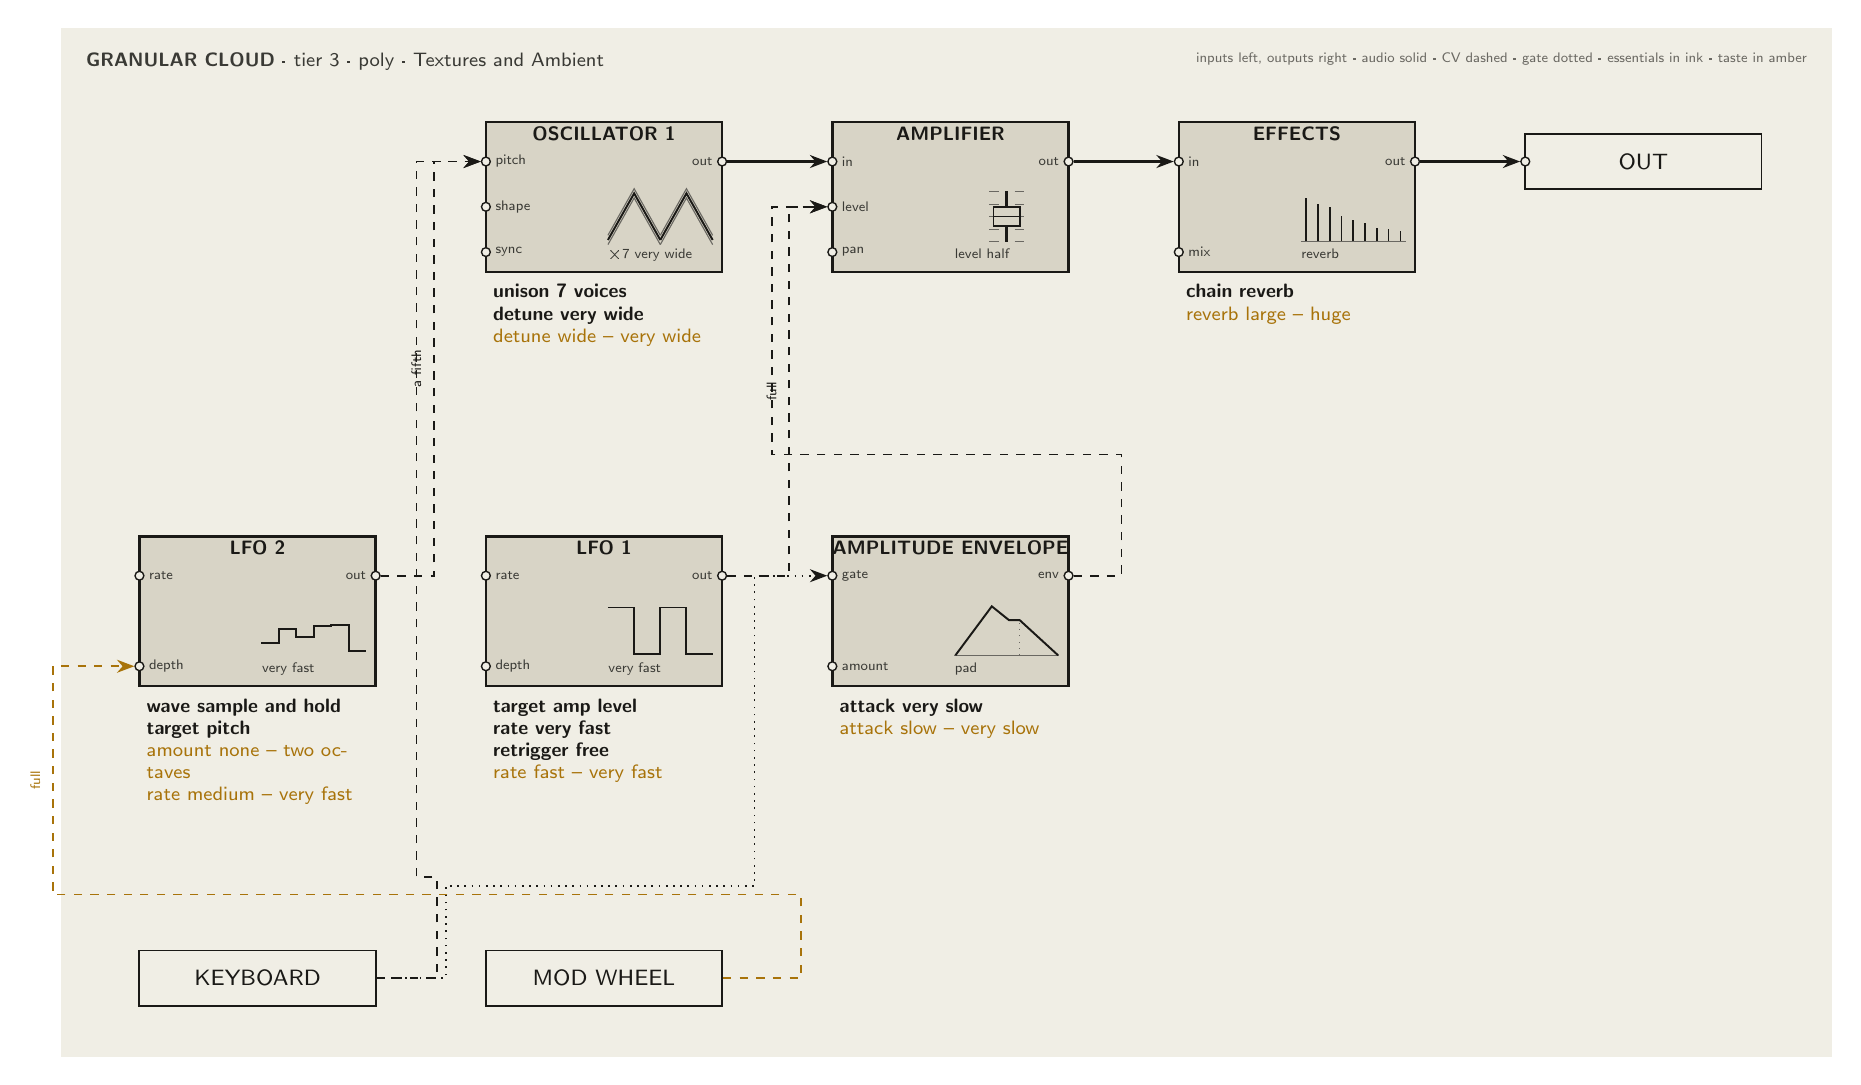
\begin{tikzpicture}
\begin{scope}[on background layer]\fill[paper] (-2.5,-10.92) rectangle (20.0,2.15);\end{scope}
\node[block, minimum height=1.9cm] (osc1) at (4.4,0.0) {};
\node[title] at (osc1.north) {OSCILLATOR 1};
\node[jack] (osc1-pitch) at (2.9000000000000004,0.44999999999999996) {};
\node[plabel] at (2.9800000000000004,0.44999999999999996) {pitch};
\node[jack] (osc1-shape) at (2.9000000000000004,-0.125) {};
\node[plabel] at (2.9800000000000004,-0.125) {shape};
\node[jack] (osc1-sync) at (2.9000000000000004,-0.7) {};
\node[plabel] at (2.9800000000000004,-0.7) {sync};
\node[jack] (osc1-out) at (5.9,0.44999999999999996) {};
\node[olabel] at (5.82,0.44999999999999996) {out};
\begin{scope}
\draw[inkthree, line width=0.4pt] (4.450,-0.487) -- (4.783,0.105) -- (5.115,-0.487);
\draw[inkthree, line width=0.4pt] (5.115,-0.487) -- (5.447,0.105) -- (5.780,-0.487);
\draw[inkthree, line width=0.4pt] (4.450,-0.605) -- (4.783,-0.013) -- (5.115,-0.605);
\draw[inkthree, line width=0.4pt] (5.115,-0.605) -- (5.447,-0.013) -- (5.780,-0.605);
\draw[ink, line width=0.7pt] (4.450,-0.546) -- (4.783,0.046) -- (5.115,-0.546);
\draw[ink, line width=0.7pt] (5.115,-0.546) -- (5.447,0.046) -- (5.780,-0.546);
\node[font=\tiny, text=inktwo, anchor=north west, inner sep=0pt] at (4.450,-0.650) {×7 very wide};
\end{scope}
\node[settings] at (2.95,-1.0699999999999998) {\textbf{unison 7 voices} \\ \textbf{detune very wide} \\ \textcolor{amber}{detune wide -- very wide}};
\node[block, minimum height=1.9cm] (amp) at (8.8,0.0) {};
\node[title] at (amp.north) {AMPLIFIER};
\node[jack] (amp-in) at (7.300000000000001,0.44999999999999996) {};
\node[plabel] at (7.380000000000001,0.44999999999999996) {in};
\node[jack] (amp-level) at (7.300000000000001,-0.125) {};
\node[plabel] at (7.380000000000001,-0.125) {level};
\node[jack] (amp-pan) at (7.300000000000001,-0.7) {};
\node[plabel] at (7.380000000000001,-0.7) {pan};
\node[jack] (amp-out) at (10.3,0.44999999999999996) {};
\node[olabel] at (10.22,0.44999999999999996) {out};
\begin{scope}
\draw[ink, line width=1.2pt] (9.515,-0.570) -- (9.515,0.070);
\draw[inkthree, line width=0.3pt] (9.295,-0.570) -- (9.415,-0.570) (9.615,-0.570) -- (9.735,-0.570);
\draw[inkthree, line width=0.3pt] (9.295,-0.410) -- (9.415,-0.410) (9.615,-0.410) -- (9.735,-0.410);
\draw[inkthree, line width=0.3pt] (9.295,-0.250) -- (9.415,-0.250) (9.615,-0.250) -- (9.735,-0.250);
\draw[inkthree, line width=0.3pt] (9.295,-0.090) -- (9.415,-0.090) (9.615,-0.090) -- (9.735,-0.090);
\draw[inkthree, line width=0.3pt] (9.295,0.070) -- (9.415,0.070) (9.615,0.070) -- (9.735,0.070);
\fill[slab, draw=ink, line width=0.6pt] (9.345,-0.370) rectangle (9.685,-0.130);
\draw[ink, line width=0.5pt] (9.345,-0.250) -- (9.685,-0.250);
\node[font=\tiny, text=inktwo, anchor=north west, inner sep=0pt] at (8.850,-0.650) {level half};
\end{scope}
\node[block, minimum height=1.9cm] (fx) at (13.200000000000001,0.0) {};
\node[title] at (fx.north) {EFFECTS};
\node[jack] (fx-in) at (11.700000000000001,0.44999999999999996) {};
\node[plabel] at (11.780000000000001,0.44999999999999996) {in};
\node[jack] (fx-mix) at (11.700000000000001,-0.7) {};
\node[plabel] at (11.780000000000001,-0.7) {mix};
\node[jack] (fx-out) at (14.700000000000001,0.44999999999999996) {};
\node[olabel] at (14.620000000000001,0.44999999999999996) {out};
\begin{scope}
\draw[inkthree, line width=0.3pt] (13.250,-0.561) -- (14.580,-0.561);
\draw[ink, line width=0.6pt] (13.317,-0.561) -- (13.317,-0.018);
\draw[ink, line width=0.6pt] (13.466,-0.561) -- (13.466,-0.095);
\draw[ink, line width=0.6pt] (13.616,-0.561) -- (13.616,-0.133);
\draw[ink, line width=0.6pt] (13.765,-0.561) -- (13.765,-0.246);
\draw[ink, line width=0.6pt] (13.915,-0.561) -- (13.915,-0.296);
\draw[ink, line width=0.6pt] (14.065,-0.561) -- (14.065,-0.335);
\draw[ink, line width=0.6pt] (14.214,-0.561) -- (14.214,-0.394);
\draw[ink, line width=0.6pt] (14.364,-0.561) -- (14.364,-0.408);
\draw[ink, line width=0.6pt] (14.514,-0.561) -- (14.514,-0.429);
\node[font=\tiny, text=inktwo, anchor=north west, inner sep=0pt] at (13.250,-0.650) {reverb};
\end{scope}
\node[settings] at (11.750000000000002,-1.0699999999999998) {\textbf{chain reverb} \\ \textcolor{amber}{reverb large -- huge}};
\node[block, minimum height=1.9cm] (lfo2) at (0.0,-5.26) {};
\node[title] at (lfo2.north) {LFO 2};
\node[jack] (lfo2-rate) at (-1.5,-4.81) {};
\node[plabel] at (-1.42,-4.81) {rate};
\node[jack] (lfo2-depth) at (-1.5,-5.959999999999999) {};
\node[plabel] at (-1.42,-5.959999999999999) {depth};
\node[jack] (lfo2-out) at (1.5,-4.81) {};
\node[olabel] at (1.42,-4.81) {out};
\begin{scope}
\draw[ink, line width=0.7pt] (0.050,-5.665) -- (0.272,-5.665) -- (0.272,-5.484) -- (0.493,-5.484) -- (0.493,-5.587) -- (0.715,-5.587) -- (0.715,-5.448) -- (0.937,-5.448) -- (0.937,-5.436) -- (1.158,-5.436) -- (1.158,-5.767) -- (1.380,-5.767);
\node[font=\tiny, text=inktwo, anchor=north west, inner sep=0pt] at (0.050,-5.910) {very fast};
\end{scope}
\node[settings] at (-1.45,-6.33) {\textbf{wave sample and hold} \\ \textbf{target pitch} \\ \textcolor{amber}{amount none -- two octaves} \\ \textcolor{amber}{rate medium -- very fast}};
\node[block, minimum height=1.9cm] (lfo1) at (4.4,-5.26) {};
\node[title] at (lfo1.north) {LFO 1};
\node[jack] (lfo1-rate) at (2.9000000000000004,-4.81) {};
\node[plabel] at (2.9800000000000004,-4.81) {rate};
\node[jack] (lfo1-depth) at (2.9000000000000004,-5.959999999999999) {};
\node[plabel] at (2.9800000000000004,-5.959999999999999) {depth};
\node[jack] (lfo1-out) at (5.9,-4.81) {};
\node[olabel] at (5.82,-4.81) {out};
\begin{scope}
\draw[ink, line width=0.7pt] (4.450,-5.214) -- (4.783,-5.214) -- (4.783,-5.806) -- (5.115,-5.806) -- (5.115,-5.214) -- (5.447,-5.214) -- (5.447,-5.806) -- (5.780,-5.806);
\node[font=\tiny, text=inktwo, anchor=north west, inner sep=0pt] at (4.450,-5.910) {very fast};
\end{scope}
\node[settings] at (2.95,-6.33) {\textbf{target amp level} \\ \textbf{rate very fast} \\ \textbf{retrigger free} \\ \textcolor{amber}{rate fast -- very fast}};
\node[block, minimum height=1.9cm] (aenv) at (8.8,-5.26) {};
\node[title] at (aenv.north) {AMPLITUDE ENVELOPE};
\node[jack] (aenv-gate) at (7.300000000000001,-4.81) {};
\node[plabel] at (7.380000000000001,-4.81) {gate};
\node[jack] (aenv-amount) at (7.300000000000001,-5.959999999999999) {};
\node[plabel] at (7.380000000000001,-5.959999999999999) {amount};
\node[jack] (aenv-out) at (10.3,-4.81) {};
\node[olabel] at (10.22,-4.81) {env};
\begin{scope}
\draw[inkthree, line width=0.3pt] (8.850,-5.821) -- (10.180,-5.821);
\draw[ink, line width=0.7pt] (8.863,-5.821) -- (9.325,-5.199) -- (9.542,-5.373) -- (9.678,-5.373) -- (10.167,-5.821);
\draw[inkthree, line width=0.3pt, dotted] (9.678,-5.821) -- (9.678,-5.373);
\node[font=\tiny, text=inktwo, anchor=north west, inner sep=0pt] at (8.850,-5.910) {pad};
\end{scope}
\node[settings] at (7.3500000000000005,-6.33) {\textbf{attack very slow} \\ \textcolor{amber}{attack slow -- very slow}};
\node[perf] (key) at (0.0,-9.92) {KEYBOARD};
\node[perf] (wheel) at (4.4,-9.92) {MOD WHEEL};
\node[perf, fill=paper] (out) at (17.6,0.44999999999999996) {OUT}; \node[jack] (out-in) at (16.1,0.44999999999999996) {};
\draw[wire,->] (osc1-out) -- (amp-in);
\draw[wire,->] (amp-out) -- (fx-in);
\draw[wire,->] (fx-out) -- (out-in);
\draw[modwire,->] (lfo1-out) -- (6.750000000000001,-4.81) -- (6.750000000000001,-0.125) -- (amp-level);
\node[font=\tiny, text=ink, anchor=south, inner sep=1pt, rotate=90] at (6.630000000000001,-2.4675) {full};
\draw[modwire,->] (lfo2-out) -- (2.2400000000000007,-4.81) -- (2.2400000000000007,0.44999999999999996) -- (osc1-pitch);
\node[font=\tiny, text=ink, anchor=south, inner sep=1pt, rotate=90] at (2.1200000000000006,-2.1799999999999997) {a fifth};
\draw[modwire,->] (aenv-out) -- (10.97,-4.81) -- (10.97,-3.27) -- (6.530000000000001,-3.27) -- (6.530000000000001,-0.125) -- (amp-level);
\draw[modwire,->] (key.east) -- (2.28,-9.92) -- (2.28,-8.64) -- (2.0200000000000005,-8.64) -- (2.0200000000000005,0.44999999999999996) -- (osc1-pitch);
\draw[gatewire,->] (key.east) -- (2.39,-9.92) -- (2.39,-8.75) -- (6.3100000000000005,-8.75) -- (6.3100000000000005,-4.81) -- (aenv-gate);
\draw[tastewire,->] (wheel.east) -- (6.9,-9.92) -- (6.9,-8.860000000000001) -- (-2.5999999999999996,-8.860000000000001) -- (-2.5999999999999996,-5.959999999999999) -- (lfo2-depth);
\node[font=\tiny, text=amber, anchor=south, inner sep=1pt, rotate=90] at (-2.7199999999999998,-7.41) {full};
\node[anchor=north west, font=\scriptsize, text=inktwo] at (-2.3,1.95) {\textbf{GRANULAR CLOUD} · tier 3 · poly · Textures and Ambient};
\node[anchor=north east, font=\tiny, text=inkthree] at (19.8,1.95) {inputs left, outputs right · audio solid · CV dashed · gate dotted · essentials in ink · taste in amber};
\end{tikzpicture}\end{document}
